\subsection{Sprint 12: da 2024-08-19 a 2024-09-02}
\par Nel corso degli \glossario{sprint} precedenti, il team ha completato la progettazione di dettaglio sia del \glossario{front-end} che del \glossario{back-end}, raggiungendo inoltre significativi progressi nelle attività di codifica. Di conseguenza, lo sprint 12 sarà focalizzato sulla fase di testing del codice e sull'aggiornamento della documentazione.

\subsubsection{Obiettivi}
\begin{itemize}
  \item Aggiornamento del documento di \ST\ nelle seguenti sezioni:
  \begin{itemize}
    \item Diagrammi delle classi;
    \item \glossario{DTO} (Data Transfer Objects);
    \item Adapter e porte;
    \item Core dell'applicazione;
    \item Design pattern utilizzati.
  \end{itemize}
  \item Stesura verbali interni;
  \item Stesura consuntivo \glossario{sprint} 11;
  \item Miglioramento delle sezioni descrittive nel \MU; 
  \item Aggiornamento del \PdQ;
  \item Implementazione dei seguenti test \glossario{back-end}:
  \begin{itemize}
    \item Generazione del \glossario{prompt};
    \item File repository;
    \item Interazione con il \glossario{database};
    \item Autenticazione;
    \item \glossario{JSON} validator e funzioni di utilità;
    \item Services e controller.
  \end{itemize}
  \item Implementazione dei seguenti test \glossario{front-end}:
  \begin{itemize}
    \item Login dialog;
    \item Layout;
    \item CreateUpdateDictionaryModal;
    \item DictionariesListView;
    \item ChatView;
  \end{itemize}
  \item Ampliamento dei commenti del back-end;
  \item Miglioramento della funzionalità di ricerca semantica.
\end{itemize}

\begin{figure}[H]
  \centering
  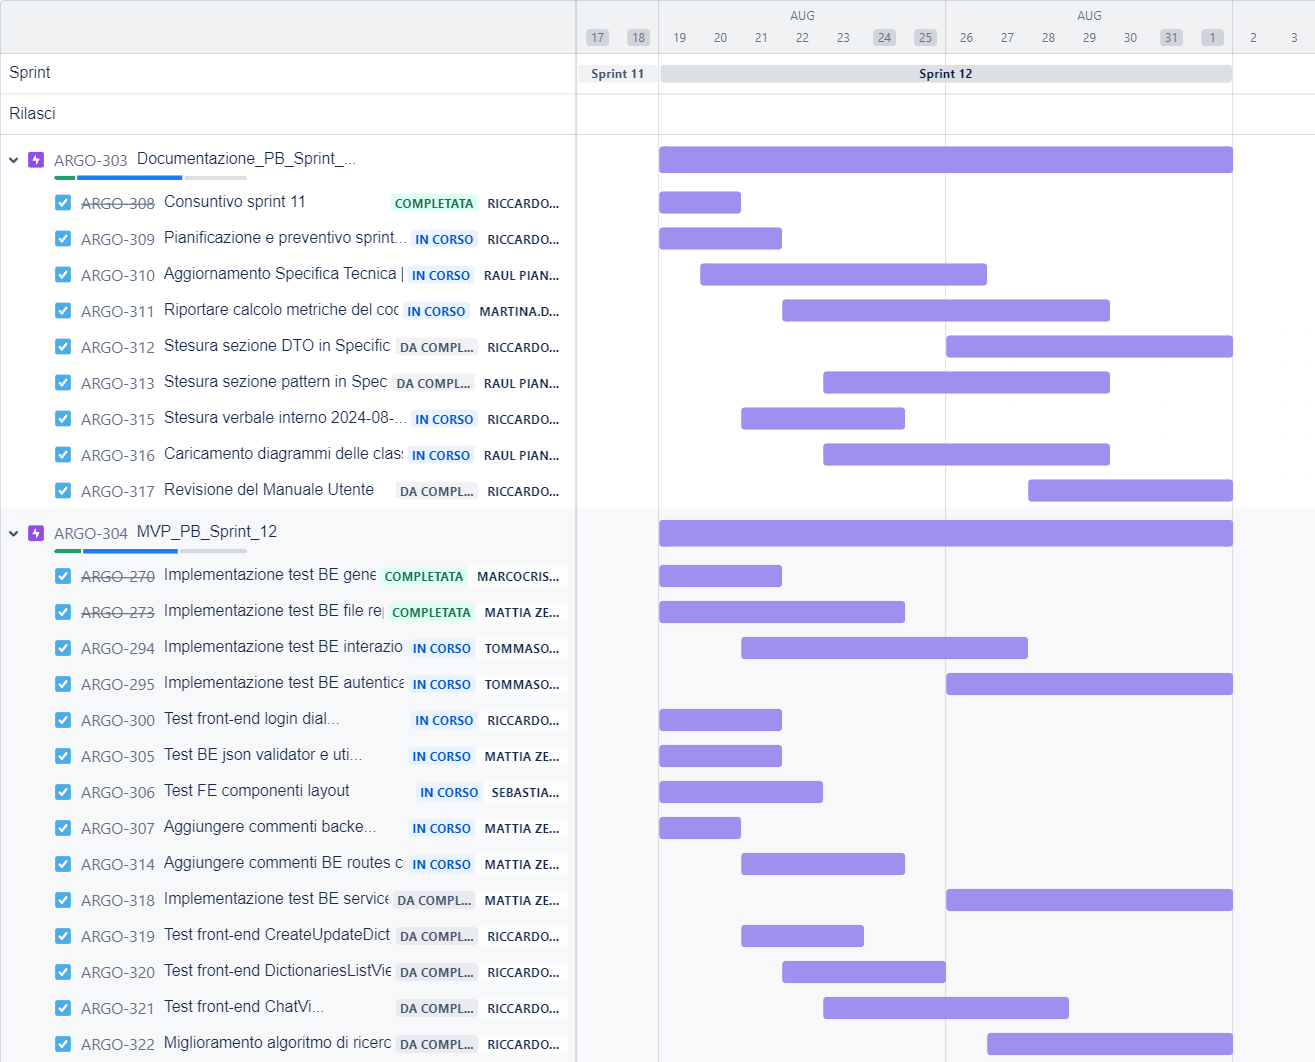
\includegraphics[width=0.90\textwidth]{assets/Pianificazione/Sprint-12/gantt.png}
  \caption{Sprint 12 - Diagramma di Gantt}\label{fig:sprint-12-gantt}
\end{figure}

